%%%%%%%%%%%%%%%%%%%%%%%%%%%%%%%%%%%%%%%%%%%%%%%%%%%%%%%%%%%%%%%%%%%%
% Grundlagen
%%%%%%%%%%%%%%%%%%%%%%%%%%%%%%%%%%%%%%%%%%%%%%%%%%%%%%%%%%%%%%%%%%%%

\chapter{Preliminaries}
  \label{PR}
This chapter explains the fundamentals of graph theory and introduces definitions and notations that are used in this thesis.
\section{Basics}
Formally a graph $G = (V, E)$ consists of a finite set of vertices $V$ and a finite set of edges $E \subset V \times V$, where each edge $e_i$ connects two vertices $v_j, v_k \in V$. We state that $n := |V|$ and $m := |E|$.\\
A \textit{path} $p$ is a series of edges $(e_1, e_2,...,e_m), e_1,...,e_m \in E$. The same path can also be described as a sequence of vertices $(v_1,v_2,...,v_k)$, where for example $e_1$ connects $v_1,v_2$.
\subsection{Attributes of a graph}
\subsubsection{Directed or undirected}
A graph can be either \textit{directed} or \textit{undirected}.\\
In a \textit{directed} graph all edges $e \in E$ are described as an ordered pair of vertices $e = (u,v)$, where the first vertex is referred to the source and the second is referred to as the target vertex.\\
In an \textit{undirected} graph each edge is defined by an unordered pair of vertices $e = {u,v}$ with no definit source or target. 
\subsubsection{Weighted or unweighted}
A graph can have \textit{weighted} or \textit{unweighted} edges.\\
If a graph is defined as \textit{weighted} it's definition includes a function $w: E \rightarrow \mathbb{R}$ which assigns a weight to each edge $e \in E$. 
\subsubsection{Complete} 
A \textit{complete} graph contains an edge $e$ for every pair of vertices $v, u \in V$. \textit{Complete} graphs are denoted as $K_n$ where $n$ is the amount of vertices.\\
For an \textit{undirected} graph with $n$ vertices there exist exactly $\frac{n^2 -n}{2}$ edges. 
\subsubsection{Connected}
A graph is called \textit{connected}, if for every two vertices $v_i, v_j \in V$ there is a path from $v_i$ to $v_j$, meaning there are no unreachable vertices.
\subsubsection{Acyclic}
An \textit{acyclic} graph has no cycles, which means that there exists no path $(v_0, v_1,...,v_k)$ where $v_0 = v_k$, that is to say that for every path in the graph the start vertex and end vertex can not be the same.
\subsubsection{Bipartite}
A graph is called \textit{bipartite} if its vertices $V$ can be divided in two subsets $V_0, V_1 \subset V$ such that the intersecting set is empty, $V_0 \cap V_1 = \emptyset$, the union of the set is the complete set of vertices, $V_0 \cup V_1 = V$, and each edge $(u,v) \in E$ connects one vertice from $V_0$ with one vertice from $V_1$, $v \in V_0$ and $u \in V_1$.
\subsubsection{Trees and forests}
A \textit{tree} is a \textit{connected}, \textit{acyclic} graph.\\
A \textit{forest} is an graph consisting of several tree graphs, meaning it is not \textit{connected} but each connected subgraph is \textit{acyclic}.
\begin{figure}[h!]
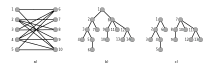
\includegraphics[width= \textwidth]{figures/BipartiteTreeForest.png}
\label{BTF}
\caption{a) A bipartite graph, b) a tree, c) a forest}
\end{figure}

\subsubsection{Planar}
A graph is \textit{planar} if it can be drawn in a way that no two edges $e_i, e_j \in E$ cross. \\
A graph is \textit{maximal planar} if no edge can be added to the graph without loosing the planarity. $K_4$ is the biggest \textit{complete} graph that is planar.\\
The drawing of a graph is referred to as \textit{plane} if no edges cross. Note that a graph can be \textit{planar} but a particular embedding of the graph is not necessarily \textit{plane}.
\begin{figure}[h!]
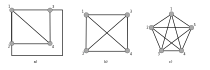
\includegraphics[width =\textwidth]{figures/PlanarPlaneGraphs.png}
\label{PPG}
\caption{a) A planar and plane graph, b) a planar but not plane graph, c) a neither plane nor planar graph}
\end{figure}
\newpage
\section{Linear layouts}
%\cite{dujmovic2004linear}
A linear layout of a graph is a layout in which all the vertices $V \in G$ are positioned along a line called the \textit{spine}.\\
The order in which these vertices are placed on the spine, is described by a bijective function $$\sigma : V \mapsto \{1,...,n\} $$. This function defines a relation where the following statements hold:
\begin{itemize}
\item Antisymmetry: if $\sigma(v_0) \leq sigma(v_1)$ and $\sigma(v_1) \leq \sigma(v_1)$ then $v_0 = v_1$
\item Transitivity: if $\sigma(v_0) \leq \sigma(v_1)$ and $\sigma(v_1) \leq \sigma(v_2)$ then $\sigma(v_0) \leq \sigma(v_2)$
\item Connexity: either $\sigma(v_0) \leq \sigma(v_1)$ or $\sigma(v_1) \leq \sigma(v_1)$ is true
\end{itemize}
These relation properties make the relation a \textit{total order} and the set of vertices a \textit{linearly ordered set}.\\
The edges of the graph are sorted into $p$ disjoint subsets $E_p \subset E$ by the surjective function 
$$ \pi: E \rightarrow \{1,..,p\} $$ making it a partition of $E$.\\
In the linear layout each subset represents one half-plane, delimited by the spine, on which all the edges will be placed.
In order to make it possible to draw these graphs in a 2D setting each half-plane is usually colored differently which is why the subsets are sometimes also referred to as \textit{colors}.\\
The following sections explain which requirements the order of vertices and the assignment of edges follow.
\subsection{Stack layouts}
For a stack layout, sometimes also referred to as a \textit{book embedding}, $\mathcal{E}(G,p)$ the vertices of the graph $G$ need to be ordered in a way that now two edges $e_i, e_j$ assinged to the same subset (called \textit{pages} of a book embedding) $\pi(e_i) = \pi(e_j)$ cross, that is to say each each half-plane contains a \textit{planar} subgraph.\\
The \textit{book thickness} or \textit{stack number} of a graph defines the minimal number of pages that is needed to embed the graph in such a layout.\\
In the past remarkable insights about these embeddings could be gained:
\textcolor{red}{Insights}\\
\subsection{Queue layouts}
For a queue layout $\mathcal{Q}(G,q)$ the order of the vertices is chosen so that no two edges $e_i, e_j$ where $\pi(e_i) = \pi(e_j)$ are nested. Two edges $e_i, e_j$ are nested if both endpoints of edge $e_i$ are between both endpoints of edge $e_j$, as shown in \textcolor{red}{Figure somewhat}.
\begin{figure}[!h]
\begin{center}
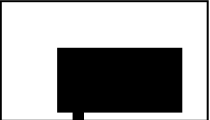
\includegraphics[width=1\textwidth]{figures/Platzhalter.png}
\caption{Crossing and Nesting Edges}
\label{img:plzhltr}
\end{center}
\end{figure}
Similar to the \textit{book thickness} in stack layouts a queue layout has a \textit{queue number} that states in how many queues the graph can be embedded minimally.\\
\textcolor{red}{research}.
\subsection{Further restrictions}
In addition to either being a stack or a queue, each half plane can be restricted further to have a special graph structure:
\subsubsection{Tree or forest subgraphs}
A half plane or page of the layout has to be in the structure of a \textit{tree} or \textit{forest}, meaning that it is \textit{acyclic} and in the case of a \textit{tree} also connected.
\subsubsection{Dispersible subgraphs}
A \textit{dispersible} subgraph is a graph in which no two edges share one endpoint. This kind of graph is also called a \textit{matching}.
\begin{figure}[!h]
\begin{center}
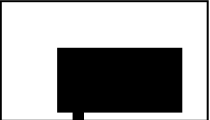
\includegraphics[width=1\textwidth]{figures/Platzhalter.png}
\caption{Dispersible Subgraphs}
\label{img:plzhltr}
\end{center}
\end{figure} 
\newpage
\section{Boolean satisfiability problem}
In 2015 the Algorithms Research Group of University of Tübingen proposed a new method to compute linear layouts automatically. \\
They found a way to formulate linear layouts as SAT-Formulas and used SAT-Solvers in order to get the order of vertices $V$ and the assignments of edges to stacks (or queues) efficiently.\\
The following section provides the theory behind SAT-formulas and  a rough explanation of how the properties of a linear layout are translated.
\subsection{SAT problem}
SAT is short for satisfiability and means the \textit{Boolean satisfiability problem}, which is the problem of determining whether there exists an assignment of truth values that satisfies a Boolean formula in \textit{conjunctive normal form} (see below). This problem is np-complete. \\
A Boolean formula consists of variables and operators ($\land$ for AND, $\lor$ for OR, $\neg$ for negation) which may be organized by parantheses. A formula is satisfiable if there exists an assignment of truth variables \textbf{true} and \textbf{false} to the variables, such that the formula evaluates to \textbf{true}.\\
Problems for SAT are formulated in \textit{conjunctive normal form}.
This means that the formula is a conjunction of clauses, where each clause is a disjunction of variables. That is to say the variables in a clause are connected by OR ($\lor$) and the clauses are connected by AND ($\land$). The opposite of CNF would be the \textit{disjunctive normal form}, where the formula is disjunction of clauses which are are conjunction of variables. 
\begin{figure}[!h]
\begin{center}
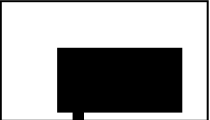
\includegraphics[width=1\textwidth]{figures/Platzhalter.png}
\caption{Sat formula?}
\label{img:plzhltr}
\end{center}
\end{figure}
\subsection{The linear layout as a SAT instance}
Let $G=(V,E)$ be the graph, and $\mathcal{F}(G,p)$ the corresponding linear layout. In this case $\mathcal{F}(G,p)$ might either be a stack embedding $\mathcal{E}(G,p)$ or queue embedding $\mathcal{Q}(G,q)$.\\
